  \documentclass[12pt,oneside]{article}

%%%%%%%%%%%%%%%%%%%%%%%%%%%%
%%   Zusaetzliche Pakete  %%
%%%%%%%%%%%%%%%%%%%%%%%%%%%%
\usepackage{acronym}
\usepackage{enumerate}
\usepackage{a4wide}
\usepackage{fancyhdr}
\usepackage{graphicx}
\usepackage{palatino}
\usepackage{blindtext}
\usepackage{multirow}
\usepackage[ruled,longend]{algorithm2e}
\usepackage{float}
\usepackage{amsmath}
\usepackage{amssymb}
\usepackage{listings}
\usepackage{tocbibind}
\usepackage{dirtytalk}
%folgende Zeile auskommentieren für englische Arbeiten
\usepackage[ngerman]{babel}

\usepackage[bookmarks]{hyperref}
\usepackage[T1]{fontenc}
\usepackage[utf8]{inputenc}
\usepackage[a-1b]{pdfx}
\usepackage[justification=centering]{caption}
%\usepackage[style=unsrt,natbib=true,backend=biber]{biblatex}
\usepackage{csquotes}
\usepackage{url}
%\usepackage{subfigure}
\usepackage[utf8]{inputenc}
\usepackage[T1]{fontenc}
% Layout corrections (Schusterjungen)
\clubpenalty = 10000 
% Layout corrections (Hurenkinder) 
\widowpenalty = 10000 
\displaywidowpenalty = 10000

% Figures
\usepackage{caption}
\usepackage[hypcap=true,labelformat=simple]{subcaption}
\renewcommand{\thesubfigure}{(\alph{subfigure})}

% Tables
\usepackage{booktabs} 

\usepackage[backend=biber,style=numeric]{biblatex}
\addbibresource{literatur.bib}


% Newcommand TODO (red in text)
\newcommand{\todo}[1]{\textcolor{red}{TODO: #1}}

% Newcommand TODOM (red at border)
\newcommand{\todom}[1]{\marginpar{\parbox{1.5cm}{\textcolor{red}{TODO:\\ #1}}}}




%%%%%%%%%%%%%%%%%%%%%%%%%%%%%%
%% Definition der Kopfzeile %%
%%%%%%%%%%%%%%%%%%%%%%%%%%%%%%

\pagestyle{fancy}
\fancyhf{}
\cfoot{\thepage}
\setlength{\headheight}{16pt}

%%%%%%%%%%%%%%%%%%%%%%%%%%%%%%%%%%%%%%%%%%%%%%%%%%%%%
%%  Definition des Deckblattes und der Titelseite  %%
%%%%%%%%%%%%%%%%%%%%%%%%%%%%%%%%%%%%%%%%%%%%%%%%%%%%%

\newcommand{\HSFTitle}[8]{

  \thispagestyle{empty}
\begin{center}
    
\includegraphics[width=0.8\textwidth]{logo.eps} \\
    \vspace*{\stretch{1}}
    \end{center}

  %\vspace*{\stretch{1}}
  {\parindent0cm
  \rule{\linewidth}{.7ex}}
  \begin{center}
    \vspace*{\stretch{1}}
    \sffamily\bfseries\Huge
    #1\\
    \vspace*{\stretch{1}}
    \sffamily\bfseries\large
    #3
    \vspace*{\stretch{1}}
  \end{center}
  \rule{\linewidth}{.7ex}

  \vspace*{\stretch{2}}
  \begin{center}
    \Large #2 am #5 der HAW Fulda \\
    \vspace*{\stretch{1}} 
    \large Matrikelnummer:  #4 \\[1mm]
    \large Erstbegutachtung:  #7 \\[1mm]
    \large Zweitbegutachtung:  #8 \\[1mm]
    \vspace*{\stretch{1}}
    \large Eingereicht am #6
  \end{center}
}


%%%%%%%%%%%%%%%%%%%%%%%%%%%%
%%  Beginn des Dokuments  %%
%%%%%%%%%%%%%%%%%%%%%%%%%%%%


\begin{document}
 
 

 \HSFTitle
      {Entwicklung und Implementierung eines Modells zur Erfassung und Bewertung der User Experience am Beispiel der Anwendung eDok des LWV Hessene }        % Titel der Arbeit
      {Bachelorarbeit} % Typ der Arbeit
      {Ali Alkhiami}          % Vor- und Nachname des Autors
      {844620}
      {Fachbereich AI}  % Name des FBs
      {05.mm.yyyy}        % Tag der Abgabe
      {Prof. Dr. Alexander Gepperth}     % Name des Erstgutachters
      {Prof. Dr. Dr. YYY}    % Name des Zweitgutachters

  \clearpage

\lhead{}
    \setcounter{page}{1}
\tableofcontents
%--------------------------------------------------------------------------------------------------------------------------------------------------------------------------------------%
\section{Abkürzungsverzeichnis}
\addcontentsline{toc}{section}{Abkürzungsverzeichnis} % Fügt das Abkürzungsverzeichnis zum Inhaltsverzeichnis hinzu
\begin{acronym}[hyperlinks]
\acro{UX}{User Experience}
\acro{LWV}{Landeswohlfahrtsverband}
\acro{SUS}{System Usability Scale}
\acro{UEQ}{User Experience Questionnaire}
\acro{UI}{User Interface}
\acro{UI}{eDok}{elektronische Dokumentenerstellung}
\end{acronym}
%--------------------------------------------------------------------------------------------------------------------------------------------------------------------------------------%
\section{Abstract}
   Diese Arbeit widmet sich der Entwicklung und Implementierung eines Modells zur umfassenden Erfassung und Bewertung der User Experience (UX) am Beispiel der Anwendung eDok des Landeswohlfahrtsverbands Hessen (LWV Hessen). Angesichts der zunehmenden Bedeutung von UX
in der Softwareentwicklung wird zunächst das Konzept der UX detailliert erläutert, gefolgt von einer kritischen Analyse gängiger Methoden zur UX-Erfassung. Im Mittelpunkt steht die Entwicklung eines Modells, das es ermöglicht, spezifische UX-Aspekte systematisch zu erfassen und zu bewerten. 
Das Modell zielt darauf ab, eine automatisierte und kontinuierliche Sammlung relevanter Daten sicherzustellen, um daraus fundierte Erkenntnisse über die Nutzererfahrung abzuleiten. Ein besonderer Schwerpunkt liegt dabei auf der Analyse, wie sich die UX durch fortlaufende Weiterentwicklungen und funktionale Erweiterungen der Software verändert.
 Zusätzlich wird die technische Umsetzung des Modells beschrieben, einschließlich der Softwarearchitektur und der Implementierung von Mechanismen zur Anonymisierung der erfassten Daten, um den Schutz der Privatsphäre der Nutzer*innen zu gewährleisten. Diese Anonymisierung ist essenziell, um ethischen Standards und datenschutzrechtlichen 
Vorgaben zu entsprechen. Die Arbeit schließt mit einer umfassenden Bewertung der Ergebnisse und gibt einen Ausblick auf mögliche Weiterentwicklungen des Modells. Hierbei wird insbesondere auf die Möglichkeit eingegangen, das Modell auf andere behördliche Anwendungen zu übertragen und damit eine breitere Anwendungsperspektive zu eröffnen.
%--------------------------------------------------------------------------------------------------------------------------------------------------------------------------------------%
\section{Einleitung}
UX (User Experience) ist ein fortlaufendes Forschungsfeld im Bereich der Mensch-Computer-Interaktion (HCI). Es begann an Bedeutung zu gewinnen, als Anwendungen immer komplexer und anspruchsvoller wurden. Mit der zunehmenden Verbreitung und Nutzung des Internets und der digitalen Welt wird UX (User Experience) immer wichtiger. Da immer mehr Menschen digitale Produkte und Dienste nutzen, steigt die Bedeutung von Benutzerfreundlichkeit und einem positiven Nutzererlebnis. Produkte, die sich durch eine intuitive Bedienung und ein ansprechendes Design auszeichnen, setzen sich im Wettbewerb durch und steigern die Nutzerzufriedenheit nachhaltig.

Heutzutage gibt es oft mehrere Softwarelösungen für ein digitales oder reales Problem. Aus diesem Grund spielt UX und Benutzerfreundlichkeit eine entscheidende Rolle bei der Auswahl eines Produkts. Ein gut gestaltetes Nutzererlebnis kann den Unterschied ausmachen, ob sich Benutzer für eine bestimmte Lösung entscheiden oder zu einem anderen Produkt wechseln.

Die meisten Experten und wissenschaftlichen Arbeiten sind sich einig, dass UX (User Experience) noch ein relativ junges Forschungsfeld ist. Aufgrund der dynamischen und subjektiven Natur des Themas konnte bisher keine einheitliche Definition festgelegt werden. Dies bietet jedoch den Vorteil, das Thema aus verschiedenen Blickwinkeln betrachten zu können und unterschiedliche Meinungen zu berücksichtigen. Dadurch entsteht ein breiteres und tieferes Verständnis für das Konzept der UX, was der weiteren Entwicklung der Disziplin zugutekommt.
Auf der Kehrseite erschweren unterschiedliche Hintergründe und Fachvokabulare den Fortschritt.\cite{glanznig}

UX/UI tretten in vielen Jobportalen und auf verschiedenen Social Media-Plattformen auf. Auf den ersten Blick klingt er oft nach reinen Frontend- oder Design-Aktivitäten. Doch dahinter verbirgt sich weit mehr, als man zunächst annehmen könnte. UX/UI umfasst nicht nur das visuelle Design, sondern auch umfassende Überlegungen zur Benutzerfreundlichkeit, zum Interaktionsdesign und zum gesamten Nutzererlebnis – Aspekte, die für den Erfolg eines Produkts von entscheidender Bedeutung sind.

Hassenzahl und Tractinsky haben in Ihre Arbeit User experience – a research agenda UX  erlautert, dass \say{User Experience (UX) ist ein interessantes Phänomen: Es wurde von der HCI-Community schnell angenommen, aber oft kritisiert, da es vage und schwer fassbar ist. Der Begriff umfasst verschiedene Bedeutungen (Forlizzi und Battarbee 2004), von klassischer Usability bis hin zu Schönheit, hedonischen, affektiven und erfahrungsbasierten Aspekten der Technologienutzung\protect \footnote{Eigene Übersetzung}.}\cite{research}




\subsection{Motivation}

Die Nutzung des Internets ist in den letzten Jahren zu einem festen Bestandteil des Alltags der deutschsprachigen Bevölkerung geworden. Laut der ARD/ZDF-Onlinestudie \cite{ard} verwenden mittlerweile rund 90 Prozent der Menschen ab 14 Jahren regelmäßig das Internet, wobei die mediale Internetnutzung im Jahr 2019 besonders stark zugenommen hat.

Diese Entwicklung unterstreicht die zunehmende Relevanz digitaler Medien und stellt neue Anforderungen an die Gestaltung von Nutzererlebnissen (User Experience, UX). Es wird zunehmend wichtiger, digitale Inhalte und Services so zu gestalten, dass sie den sich wandelnden Ansprüchen der Nutzer gerecht werden. UX spielt eine zentrale Rolle bei der Bewertung und Optimierung von Softwareanwendungen. Dies gilt insbesondere für behördliche Anwendungen wie eDok, das vom LWV Hessen und anderen Institutionen genutzt wird. Hier ist es entscheidend, die UX zu erfassen und zu verbessern, um die Benutzerfreundlichkeit und Effizienz der Anwendung zu steigern.

Eine besondere Herausforderung besteht darin, Bereiche innerhalb der Anwendung zu identifizieren, die ein verbessertes Design oder zusätzliche Informationen erfordern. Oft sind Nutzer unsicher, wie sie ihre Ziele innerhalb der Anwendung erreichen können oder fühlen sich von der Informationsmenge überfordert. Hier setzt das entwickelte Modell an, das die UX automatisiert erfasst und eine fundierte Analyse ermöglicht. So können gezielt Schlüsselaspekte identifiziert werden, die optimiert werden sollten, um die Nutzerzufriedenheit zu steigern.

Vor allem bei komplexen Webanwendungen wie eDok besteht ein großes Bedürfnis, kontinuierlich Feedback von den Nutzer*innen einzuholen, um deren Erfahrungen besser zu verstehen und die Anwendung kontinuierlich zu verbessern. Durch die Implementierung des entwickelten Modells wird es möglich, spezifische UX-Aspekte systematisch zu erfassen und einen umfassenden Überblick über das Nutzererlebnis zu gewinnen.

Zusätzlich führen die regelmäßige Einführung neuer Funktionen und Veränderungen in der Benutzeroberfläche zu einer dynamischen Komplexitätsentwicklung
 in verschiedenen Bereichen der Anwendung. Ein Überblick über die Entwicklung der UX im Laufe der Zeit ermöglicht eine proaktive Anpassung und Optimierung, 
sodass die Anwendung trotz zunehmender Komplexität benutzerfreundlich bleibt.

in dem Papier "User Experience Evaluation Methods in Academic and
Industrial Contexts" wurde drauf hingewiesen, dassUx bemessung und bewertung Methoden 
 ein wichtige Rolle spielen, um sicherzustellen das die Einticklung des Produkts in die Richtige Richtung geht.\cite{Virpi}

Das Modell bietet zudem Einblicke in die Effizienz bestimmter Bereiche der Anwendung und zeigt, wie sich die Komplexität im Laufe der Zeit verändert hat. Wenn eine Seite umfangreiche Änderungen erfahren hat, können die Entwickler*innen durch das Modell schnell nachvollziehen, wie sich UX- und Usability-Aspekte nach der Implementierung verändert haben und ob weitere Verbesserungen erforderlich sind.
%todo auf 15 seiten bringen
\subsection{Ziel der Arbeit}
Das Ziel dieser Arbeit ist es, zentrale Elemente der UX zu identifizieren, rausfinden wir man das bemessen und bewerten kann. 

Ein Modell zu entwickeln, das diese Elemente darstellt, um die UX innerhalb einer Anwendung erfassen und bewerten zu können. Es soll die Vorteile eines solchen Modells aufzeigen.
Die gesammelten Daten sollen anonymisiert werden, und die Ergebnisse des Modells sollen darüber Auskunft geben, wie sich die UX im Verlauf der Anwendungsentwicklung verändert hat. Zudem soll das Modell die UX an verschiedenen Stellen innerhalb der Anwendung erfassen und bewerten können. Entwickler*innen erhalten die Möglichkeit, zusätzliche Stellen zu messen oder solche zu entfernen, die mit der Zeit an Relevanz verloren haben.
\subsection{Fragestellung}
Welche spezifischen, anonymisierten Daten sind erforderlich, um die User Experience (UX) präzise und systematisch zu erfassen? Wie lassen sich diese Daten über Zeiträume hinweg analysieren, um dynamische Veränderungen zu erkennen und gezielte Optimierungsmöglichkeiten der Anwendung zu erschließen?

\section{Über der Landeswohlfahrtsverband Hessen}
Der Landeswohlfahrtsverband Hessen ist eine zentrale Organisation in Hessen, die sich für die soziale Integration und Unterstützung von Menschen mit Behinderungen einsetzt. Der Verband ist überörtlicher Träger der Eingliederungshilfe und fördert unter anderem in den Bereichen Wohnen, Bildung, Mobilität und Arbeit. Mit der Umsetzung des Bundesteilhabegesetzes und weiteren Programmen wie dem Persönlichen Budget  und dem Budget für Arbeit" unterstützt der LWV Hessen die selbstbestimmte Lebensführung und die gesellschaftliche Teilhabe der Betroffenen. Der LWV unterhält zudem Förderangebote für Kinder und Jugendliche, insbesondere für solche mit geistigen, emotionalen oder körperlichen Einschränkungen. Hierzu zählen Frühberatungsstellen, Förderschulen und Angebote zur inklusiven Beschulung. Zusätzlich ist der Verband Ansprechpartner für Menschen, die Leistungen des Sozialen Entschädigungsrechts benötigen.\subsection{Das Anlei-service GmbH}
Die ANLEI-Service GmbH ist eine Tochtergesellschaft des LWV Hessen  und bietet IT-Dienstleistungen für die Sozialverwaltung. Sie entwickelt Systeme zur Unterstützung der Antragsbearbeitung, Leistungsgewährung und Abrechnung von Sozialleistungen, insbesondere in den Bereichen Eingliederungshilfe, Sozialhilfe und Kriegsopferfürsorge. Zu den zentralen Anwendungen zählen das Integrierte Berichtssystem (IBS) für betriebswirtschaftliche Analysen und MASS zur maschinellen Abrechnung mit Einrichtungen und Trägern

\section{Über eDok}
   
eDok Dient als Service für alle aufrufenden Anwendungen zur Erstellung von barrierefreien Dokumenten
Löst das Schriftstück Erstellungssystem (SE) ab, das auf Microsoft Word und Makros basiert und integriert Doxee/Infinica als Subsystem für die Dokumentbearbeitung und Output-Generierung, sodass eine Verwendung sowohl mit Interaktiven Elementen (Bearbeitung des entstehenden Dokuments), als auch im Hintergrund (Dunkelverarbeitung) erfolgen kann
Ziel und Vision von eDok ist es, eine universelle und generelle Schnittstelle für unsere Anwendungen zur einfachen, effizienten und performanten Erstellung von barrierefreien Dokumenten, unter Einbeziehung der Daten aus unseren Fachverfahren, zu bilden
\section{Einführung in das Thema UX}
 
\subsection{was ist UX}
Die User Experience wurde in verschiedenen Büchern, von unterschiedlichen Autoren und Organisationen auf unterschiedliche Weise definiert. \cite{GOISTAI}

In der Arbeit  User experience - a research agenda haben Hassenzahl und Tractinsky\cite{research} erlautert dass HCI  Wessenschaftlicharbeit sich haupsichlich mit Verhaltensziele in der Arbeitsumgebung beschäftig hat, das wurde aber später herausgefordert z.b.: 

\say{In einem frühen Versuch, UX zu definieren, betonte Alben (1996) Schönheit (d.h. Ästhetik) als einen wichtigen Qualitätsaspekt von Technologie\protect \footnote{Eigene Übersetzung}.}\cite{research}
, Hassenzahl (2003)   argumienteiet , dass es zwei Aspekten, die für ein interaktiven Produkt betrachtet sein können, ein sind Instromintale Aspekte(Z.B Usabilty Testing) und nicht-instrumntale(hedonisch)  Aspekte.
Die Forsching in der Bereich hat in den Neunzige begonnen innerhalb der Gebiet HCI, da es noch nicht für UX ein Defintion gibt, wo alle Forschern sich einigen konnten, können wir 
verschieden sichtweisen und meinungen finden\cite{glanznig}.

Die Nielsen Norman Group definiert User Experience (UX) als die Gesamtheit aller Aspekte der Interaktion des Endnutzers mit dem Unternehmen, seinen Dienstleistungen und Produkten. Sie betonen, dass eine herausragende User Experience nicht nur die genauen Bedürfnisse des Kunden erfüllt, 
sondern auch Einfachheit und Eleganz bietet, die das Produkt angenehm in der Nutzung und im Besitz machen. Außerdem wird hervorgehoben, dass eine qualitativ hochwertige UX eine nahtlose Integration mehrerer Disziplinen erfordert, darunter Ingenieurwesen, Marketing, Grafik- und Industriedesign sowie Interface-Design \cite{nngroup}.
ISO 9241-210:2019 UX-Definition: „Die User Experience umfasst sämtliche Wahrnehmungen und Reaktionen von Nutzern, die durch die tatsächliche oder erwartete Nutzung eines Systems, Produkts oder einer Dienstleistung hervorgerufen werden.“
\cite{ISO}

Alle Definitionen stimmen darin überein, dass die UX das ganzheitliche Erleben eines Nutzers mit einem Produkt, einer Dienstleistung oder einem System umfasst und Faktoren wie Benutzerfreundlichkeit, Emotionen und Zufriedenheit berücksichtigt.
Die Literatur ist sich weitgehend einig darüber, dass die User Experience (UX) aus verschiedenen Dimensionen besteht. Häufig werden dabei insbesondere die Benutzerfreundlichkeit (Usability), die inhaltliche Relevanz, die ästhetische Wahrnehmung sowie das Vertrauen der Nutzer hervorgehoben \cite{toolbox}.
 Diese Dimensionen spielen eine zentrale Rolle bei der Gestaltung positiver Nutzererlebnisse und sind entscheidend dafür, wie effektiv und zufriedenstellend eine Anwendung wahrgenommen wird.

in dem Paper "Towards Practical User Experience Evaluation Methods" \cite{evaluationmethods} wurde rausgestellt, dass die Forschung im Bereich User Experience (UX) in der akademischen Gemeinschaft eine Vielzahl an Modellen und Frameworks hervorgebracht hat. 
Und diese Modelle adressieren die zentralen Herausforderungen von UX: ihre subjektive, stark kontextabhängige und dynamische Natur sowie die Berücksichtigung sowohl pragmatischer als auch hedonischer Faktoren, die das Nutzererlebnis beeinflussen. Gleichzeitig wird der Begriff UX auch zunehmend in der Industrie übernommen,
 jedoch beruhen die Praktiken in der Produktentwicklung nach wie vor weitgehend auf traditionellen Methoden der Usability. In diesem Beitrag wird die Notwendigkeit praxisnaher UX-Bewertungsmethoden und deren Anwendung in der Produktentwicklung in der Industrie diskutiert. Wir kommen zu dem Schluss, dass trotz der Tatsache,
 dass die Definition von UX noch weiter ausgearbeitet werden muss, viele Methoden aus der Mensch-Computer-Interaktion (HCI) und anderen Disziplinen an die spezifischen Aspekte der UX-Bewertung angepasst werden können.  \cite{evaluationmethods}

laut \cite{GOISTAI} kann man UX mit verschiedene Prespektiven sehen sieh \ref{fig:1}
\begin{figure}[b!]
\centering
 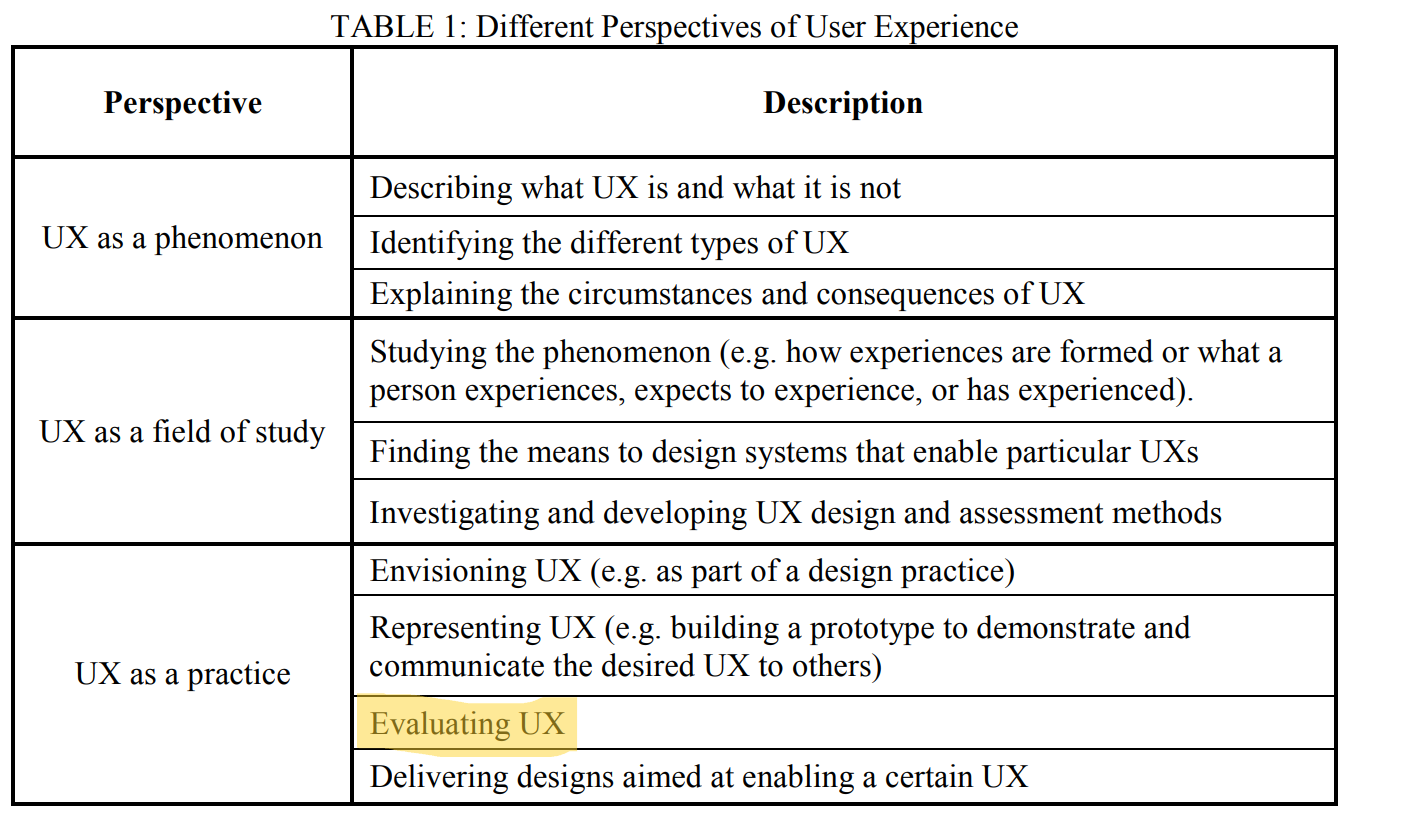
\includegraphics[width=15cm]{UXprespektiven.png}
		\caption{UX prespektiven laut \cite{GOISTAI}}
		\label{fig:1}
\end{figure}



\subsection{Bewertung von User Experience (UX)}

Laut \cite{GOISTAI} ist die bloße Messung der Anzahl von Fehlern, Klicks und der benötigten Zeit nicht ausreichend, um die User Experience (UX) adäquat zu bewerten. Es ist entscheidend zu verstehen, wie sich der Nutzer vor, während und nach der Verwendung der Anwendung oder des Produkts fühlt.
durch die Entwicklung von Webanwendung und die Enwicklung von Gaming Indusrie und und der Aufstieg des allgegenwärtigen Computings ührte zu einem Paradigmenwechsel von Effizienz hin zur Zufriedenheit der Nutzer und legte den Grundstein für die Etablierung von User Experience (UX) als eigenständigem Konzept \cite{glanznig}
\cite{Virpi} argumentiert, dass objektive Messungen wie Zeitmessung oder Fehleraufzeichnung nicht geeignet sind, um UX zu bewerten. Stattdessen sollten auch die Emotionen, Erwartungen und die Motivation des Nutzers berücksichtigt werden. UX ist zudem stark kontextabhängig und variiert je nach Einsatzgebiet und Zielgruppe.

In dem genannten Papier werden die Methoden zur UX-Bewertung nach ihrer Ausführungsart kategorisiert. Die für diese Arbeit relevante Methode ist die „Field Study“, bei der UX während eines Usability-Tests erfasst wird. Hierbei äußern die Nutzer laut denkend ihre Gedanken, und ihre Mimik wird dokumentiert, was für ein Modell nicht üblich ist. Der Usability-Test wird erweitert, um einen ganzheitlicheren Überblick über die UX zu erhalten.

Das vorgestellte Modell speichert zwar funktionale Daten wie Fehler- und Klickzähler, empfiehlt jedoch gemäß \cite{Virpi} zusätzlich eine Methode wie die Field Study in einer kontrollierten Umgebung. Somit wird nicht nur die Usability gemessen, sondern es wird auch ein Überblick über die emotionale Dimension der UX geschaffen.

Daher wurden in dieser Arbeit Methoden und Theorien zur Bewertung der Usability implementiert, welche die Anforderungen abdecken. Ergänzend dazu wurden Feedback-Pools für Seiten und Fehlermeldungen eingeführt, die optional auch Kommentare enthalten. Diese Erweiterungen ermöglichen eine detailliertere Erfassung der UX-Schnittstellen während der Usability-Tests.

Ein weiteres Ziel dieser Arbeit ist die Entwicklung eines Usability- und UX-Scores, der den Verantwortlichen eine aggregierte Übersicht bietet.

\subsection{Erweiterung der Usability-Bewertung zur UX-Analyse}

Um die Usability-Bewertung zu erweitern und die UX detaillierter darzustellen, werden folgende Daten erfasst:

\begin{itemize} \item Benutzerfeedback während der Nutzung (Survey). \item Feedback zu Fehlermeldungen (verständlich, nicht verständlich). \item Bewertung einzelner Prozessschritte zur Zufriedenheitsermittlung (Skala: sehr gut, gut, neutral, unzufrieden, sehr schlecht). \end{itemize}

Laut \cite{GOISTAI} sind UX-Bewertungsmethoden eine Erweiterung der Usability-Messungen. Usability-Bewertung konzentriert sich auf funktionale Aspekte des Systems, während UX-Bewertung zusätzlich die emotionale Dimension und die Erwartungen der Nutzer berücksichtigt.

Das Buch \cite{measuring} beschreibt verschiedene UX-Metriken \footnote{Eine Metrik ist eine Methode, um ein bestimmtes Phänomen oder eine Sache zu messen oder zu bewerten.} zur Erfassung von Nutzeraktionen. Diese Metriken können den Produktverantwortlichen helfen, fundierte Entscheidungen zu treffen.

UX-Metriken ermöglichen eine Bewertung der Interaktion zwischen Nutzer und Produkt in Bezug auf:

\begin{itemize} \item Effektivität (die Fähigkeit, eine Aufgabe zu erfüllen). \item Effizienz (der erforderliche Aufwand zur Aufgabenerfüllung). \item Zufriedenheit (das Maß an Zufriedenheit des Nutzers bei der Aufgabenbewältigung). \end{itemize}

\subsection{Usability}
 (good) usability is a precondition
for (good) UX.\cite{glanznig}
Usability bezieht sich auf die funktionalen Aspekte eines Produkts und beschreibt, wie effektiv und produktiv sich das Produkt nutzen lässt. Viele Experten sehen Usability als Teil der UX \cite{GOISTAI}. Während sich Usability auf die Fähigkeit des Nutzers konzentriert, ein System erfolgreich zu nutzen, umfasst UX auch die gesamte Nutzererfahrung und die dabei entstehenden Emotionen.
Die Nielsen Norman Group definiert \cite{nngroup} Usability als ein Qualitätsmerkmal, das bewertet, wie einfach und angenehm eine Benutzeroberfläche zu nutzen ist. Sie umfasst fünf Hauptkomponenten:
\begin{itemize}
    \item \textbf{Erlernbarkeit}: Wie leicht können Benutzer grundlegende Aufgaben beim ersten Mal ausführen?
    \item \textbf{Effizienz}: Wie schnell können Benutzer Aufgaben ausführen, nachdem sie die Schnittstelle gelernt haben?
    \item \textbf{Merkfähigkeit}: Wie einfach können Benutzer ihre Fähigkeiten wiederherstellen, wenn sie das Design nach einer Pause erneut verwenden?
    \item \textbf{Fehlerrate}: Wie viele Fehler machen Benutzer, wie schwerwiegend sind diese und wie leicht können sie sich von ihnen erholen?
    \item \textbf{Zufriedenheit}: Wie angenehm ist die Nutzung der Benutzeroberfläche?
\end{itemize}
Die ISO 9241-210 (2010) definiert die Benutzererfahrung (User Experience, UX) und die Gebrauchstauglichkeit (Usability) klar voneinander ab. Während UX sich auf die gesamte Erfahrung und Zufriedenheit der Nutzer bei der Nutzung eines Produkts konzentriert, liegt der Fokus von Usability auf der Effizienz, Effektivität und dem Zufriedenheitsgrad bei der Erledigung konkreter Aufgaben.

Im Kontext einer Webanwendung wie eDok liegt der Schwerpunkt primär auf der Dokumentenerstellung. Es ist wichtig, den Nutzern eine Möglichkeit zu bieten, schnell und effizient Dokumente mit einer gewissen Fehlertoleranz zu erstellen und zu bearbeiten. Im Anschluss daran stellt sich die Frage, wie sich die Nutzer während der Nutzung von eDok fühlen.

Usability kann hier als Indikator für die Emotionen der Nutzer dienen: Wenn die Effizienz der Anwendung abnimmt, könnte dies darauf hindeuten, dass die Anwender Schwierigkeiten haben, was zu einer erhöhten Unzufriedenheit führen kann. Im Gegensatz dazu zeigt eine gute Fehlertoleranz (z. B. durch hilfreiche Fehlermeldungen und die Möglichkeit, Fehler schnell zu beheben), dass die Nutzer trotz Fehlern ihre Ziele erreichen können. Dies trägt wiederum zur positiven Wahrnehmung der Anwendung bei und steigert die Zufriedenheit.

In diesem Arbeitskontext wird versucht, bestimmte Merkmale der Usability zu messen, zu speichern und zu bewerten. Ergänzend dazu werden weitere UX-bezogene Feedback-Services erfasst.

 


 
\subsection{Messung und Bewertung von Usabilty}

Das Buch \cite{measuring} verdeutlicht, dass UX einen breiteren Anwendungsbereich als Usability hat, da es die gesamte Nutzerinteraktion und die Emotionen berücksichtigt.






\section{Vorstellung der Funktionalitäten von eDok\protect \footnote{Die Informationen hierzu wurden teilweise von den Confluence-Seiten des LWV-Netzwerks übernommen.}}



\subsection{Was das Modul misst und darstellt}

Das Modul erfasst und stellt folgende Daten dar:

\begin{itemize} \item Heatmaps zur Visualisierung von Nutzerinteraktionen. \item Klickpositionen und -häufigkeiten. \item Feedback zu Fehlermeldungen (Like/Dislike, Verständnis der Fehlermeldung). \item Emotion-Feedback in Form von Emojis (gut, zufrieden, neutral, unzufrieden, schlecht) mit optionalen Kommentaren. \item Fehlerzähler, um die häufigsten Fehler zu identifizieren. \item Erfassung der Prozessschritte, bei denen die meisten Nutzer scheitern. \item Zeitaufwand pro Prozess, Verweildauer auf einer Seite, Zeit zur Fehlerbehebung, Prozessabbruch und Wiederaufnahme. \item Analyse der Prozesse mit der längsten Bearbeitungsdauer. \item Usability-Score und UX-Zusammenfassung über einen bestimmten Zeitraum. \end{itemize}
 

 
\section{Was führt zu optimaler UX}
 
%--------------------------------------------------------------------------------------------------------------------------------------------------------------------------------------%
\section{Erfassung der UX}
%--------------------------------------------------------------------------------------------------------------------------------------------------------------------------------------%
\section{Anonymisierte Erfassung und Behandlung der Daten}
\section{Bedeutung der Anonymisierung}
Bei der Erfassung von UX-Daten ist es entscheidend, dass die Daten anonymisiert werden, um die Privatsphäre der Nutzer*innen zu schützen und ethische Standards einzuhalten.
%--------------------------------------------------------------------------------------------------------------------------------------------------------------------------------------%
\section{Methoden zur Anonymisierung}
\begin{itemize}
\item \textbf{Pseudonymisierung}: Ersatz von personenbezogenen Daten durch Pseudonyme, sodass die Identität der Nutzer*innen nicht direkt ermittelt werden kann.
\item \textbf{Aggregation}: Zusammenfassung der Daten auf eine Ebene, die keine Rückschlüsse auf Einzelpersonen zulässt.
\end{itemize}
%--------------------------------------------------------------------------------------------------------------------------------------------------------------------------------------%
\section{Umsetzung der Anonymisierung bei eDok}
Hier wird beschrieben, wie die Anonymisierung der erhobenen UX-Daten in der Anwendung eDok umgesetzt werden kann, um den Datenschutzbestimmungen zu entsprechen.
\section{Modellarchitektur}
 
\section{Modellimplementierung}
 
\section{Schlussfolgerung und Ausblick}
 
%--------------------------------------------------------------------------------------------------------------------------------------------------------------------------------------%
 
 
  
\printbibliography
 

\end{document}

